

\section{Potential Methodological Challenges}
\label{si_section:Challenges}
Below, I provide a brief discussion of anticipated methodological challenges and constraints.

\subsection{Structure of Financing for Local Public Education}
\textbf{In order to appropriately make use of the outlined data as well as robustly define the econometric methods to be utilised in this work, an understanding of the funding structure of public school districts in the US is critical.} Public school districts in the United States are funded by a combination of federal (8.3\% in 2019), state (47\% in 2019), and local (44.8\% in 2019) revenues \cite{skinnerStateLocalFinancing2019}, with shares varying by county. This variation in public funding structure will need to be incorporated into the modelling efforts, likely through a weighted regression approach based on shares of intergovernmental versus own-source revenues \cite{skinnerStateLocalFinancing2019}. Using the data outlined, Figure \ref{fig:natl_share_rev} displays the share of public education revenue coming from three sources of intergovernmental revenue (federal, state, and local) as well as revenue from own county-level sources by state. The figure demonstrates the clear near-even split between state intergovernmental and own source revenue and the overall small share of revenue coming from federal or other local governments. The larger panel on the top left provides the summarising share at the national level. All plots share the axes as labeled in the top left panel.

\subsection{Trends over time}
According to the most recent data available from the US Congressional Research Service, the revenue share has shifted from local to state sources whereas federal funding has remained the same albeit with fluctuations over time \cite{skinnerStateLocalFinancing2019}.
\begin{figure}[ht]
    \caption{Share of Revenue from Federal, State, Local Sources \\
    }
    \centering
    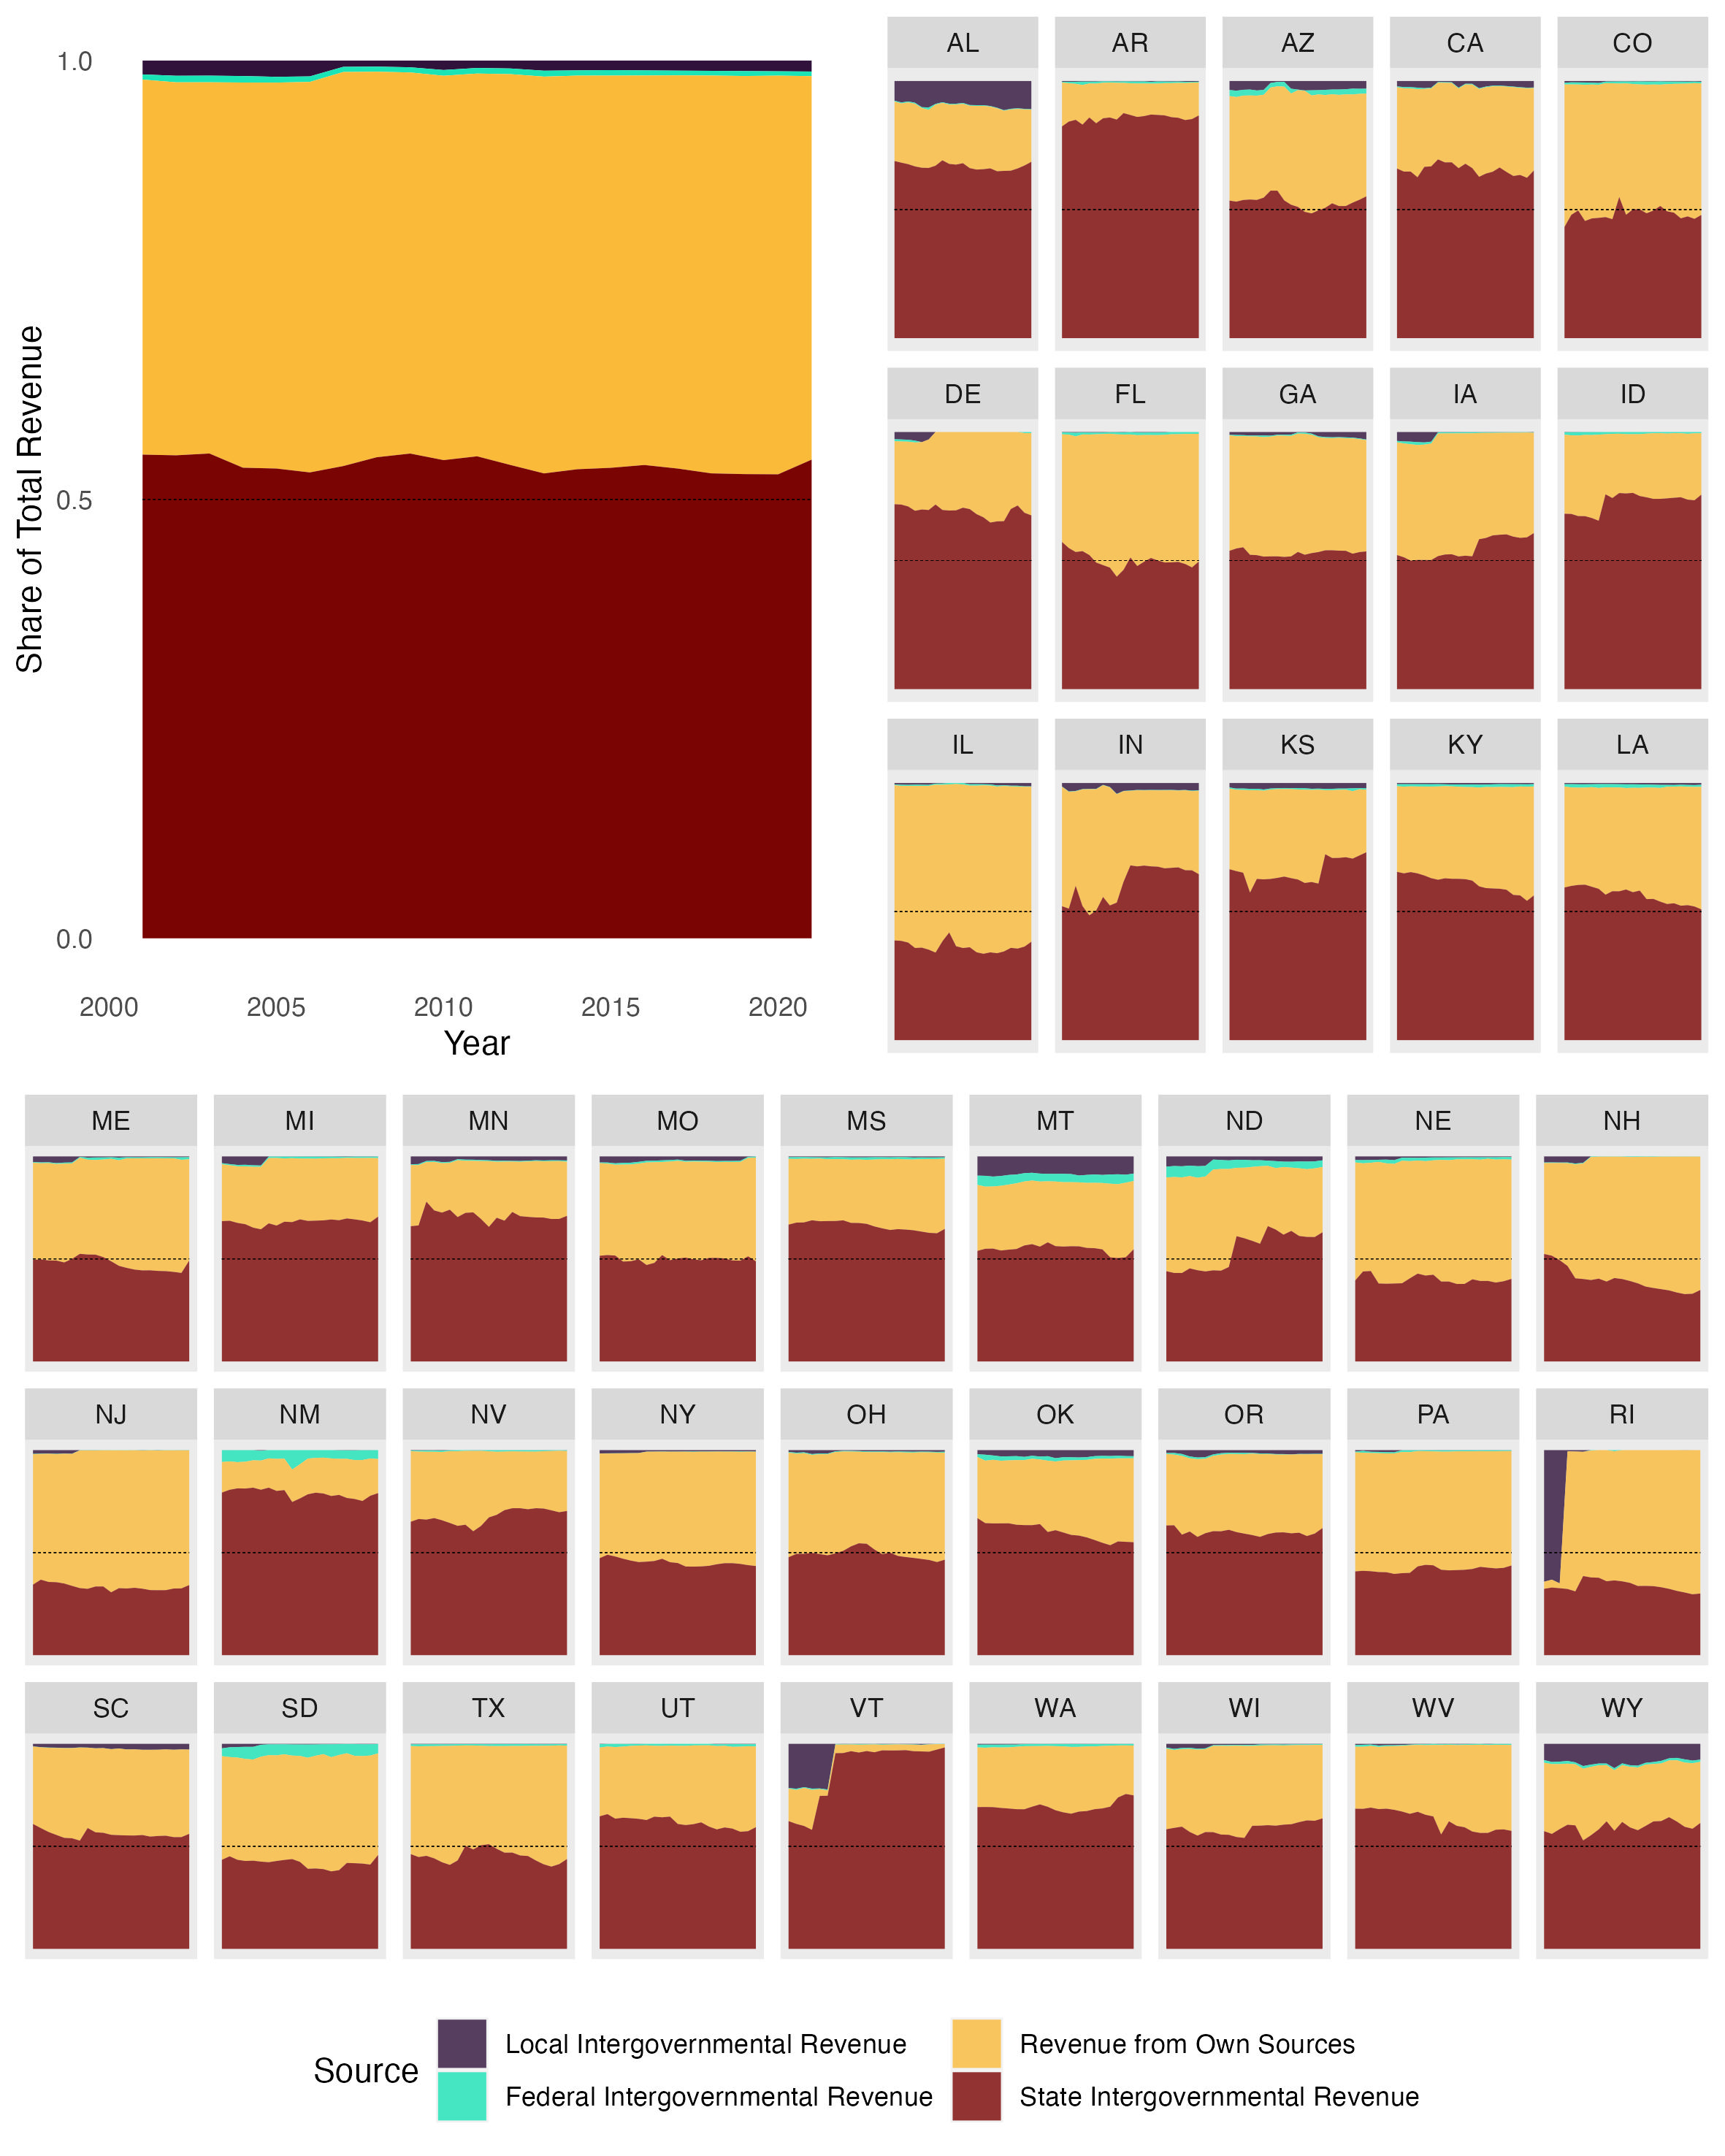
\includegraphics[scale = 0.15]{../output/natl_shares_of_revenue_by_source.jpg}
    \label{fig:natl_share_rev}
\end{figure}
\FloatBarrier

\subsection{Historical efforts to ``equalise'' US public education}
\textbf{Another factor that greatly impacts the data generating process in this study is that increasing recognition of the level of inequality of public education provision in the US has led to the implementation of several efforts to ``equalise'' public education by aiming for "per pupil" expenditure targets \cite{skinnerStateLocalFinancing2019}.} The most significant change in this respect has been the creation of Educational Service Agencies (ESAs). These ESAs are apportioned state funding to serve multiple school districts in sub-regions of each state. Most of these ESAs were established around 2007 and persist to this day. ESAs are listed by state in Table \ref{tab:si_tbl:esa_names_tbl}. Currently, there are 553 agencies nationwide in 45 states. According to the Association of Educational Service Agencies (AESA), ESAs reach over 80\% of the public school districts and well over 80\% of public and private school students. Annual budgets for ESAs total approximately \$15 billion \cite{aesaAESA2024}. Because ESA revenue and expenditure is inconsistently reported across years in our dataset, as well as attributed to individual counties despite often serving multiple, there is a significant risk that ESA expenditure is misattributed to counties in our dataset. Therefore, I exclude ESA revenue and expenditure totals from the measures of county-level expenditure and revenue at all levels of aggregation, and retain these values as possible control variables.

Preliminary investigation, both descriptive and using regression models, indicate that public expenditure from ESAs have not acted as a substitute for other revenue sources. In other words, they have not displaced intergovernmental or local school revenue. Although this fact ensures that changes in public spending on education detected in our models are not overestimated due to substitution effects from unmodelled ESA expenditure, it does risk underestimating values of actual expenditure per pupil. This remains to be resolved.

\subsection{Availability of varying local-level outcomes}

\textbf{Approaching a more "local" analysis of such challenges is often inhibited by data availability.} First, data limitations including infrequent periodicity and missingness due to strained local reporting capacity or low stringency impose a limit on the statistical power in a panel analysis. Furthermore, infrequent periodicity poses the additional challenge to interpretation when assessing the impact of industrial changes that are often subject to within-year cyclicality. 

\subsection{Structural and policy heterogeneity}

\textbf{County-level analysis of the US poses an inherent trade-off between greater local insight and requisite model complexity.} First, county-level variables are subject to unit- and time-dependent variation, which can be partly, although likely not adequately, dealt with through the incorporation of appropriate control variables and two-way fixed effects. This work will aim to incorporate consideration of spatial auto-correlation between counties to further deal with these estimation challenges. Second, and perhaps most challenging, counties are subject to state-wide regulatory, economic, and social conditions that can vary greatly across states. I aim to control for state-level variation using either an additional state-fixed effect in our regression models or state-level time trends. However, I remain wary of the residual effect of state-level heterogeneity in policy regimes and culture on our estimation results. I remain open to the idea of restricting our analysis to a smaller set of states or even a state-by-state analysis.

\subsection{Cross-Sectional Dependence}
\textbf{This latter point on state-level heterogeneity points to an additional challenge when modelling more local- or county-level variation: cross-sectional dependence.} Neighboring counties, particularly counties in the same state, will inevitably exhibit high levels of spatial dependence and auto-correlation. Adding further complication, state boundaries implicate any assumption of linearity in spatial dependence at the county level (ie. neighboring counties on either side of a state border will likely be less similar than neighboring counties within the same border).

\begin{table}
\footnotesize
\caption{\label{tab:si_tbl:esa_names_tbl}Educational Service Agencies by State}
\centering
\begin{tabular}[t]{|l|c|c|}
\hline
\textbf{State} & \textbf{ESA Name} & \textbf{\#}\\
\hline
Alabama &  & \\
\hline
Alaska & Educational Resource Center (SERRC) & 1\\
\hline
Arizona & Office County of School Superintendent & 15\\
\hline
Arkansas & Education Service Cooperative & 15\\
\hline
California & County Office of Education & 58\\
\hline
Colorado & Board of Cooperative Educational Services & 21\\
\hline
Connecticut & Regional Education Service Center & 6\\
\hline
Delaware &  & \\
\hline
Florida & Regional Consortium Service Organization & 3\\
\hline
Georgia & Regional Education Service Agency & 16\\
\hline
Hawaii &  & \\
\hline
Idaho &  & \\
\hline
Illinois & Regional Office of Education; Intermediate Service Center & 35; 3\\
\hline
Indiana & Educational Service Center & 9\\
\hline
Iowa & Area Education Agency & 9\\
\hline
Kansas & Interlocal Cooperative - Service Center & 7\\
\hline
Kentucky & Education Cooperative & 8\\
\hline
Louisiana & Special School District & 0\\
\hline
Maine &  & \\
\hline
Maryland &  & \\
\hline
Massachusetts & Educational Collaborative & 25\\
\hline
Michigan & Intermediate School District & 56\\
\hline
Minnesota & Regional Service Cooperative; Intermediate School District & 9; 4\\
\hline
Mississippi & Regional Educational Service Agency & 6\\
\hline
Missouri & Educational Service Agency & 4\\
\hline
Montana & Educational Cooperative & 2\\
\hline
Nebraska & Educational Service Unit & 17\\
\hline
Nevada &  & \\
\hline
New Hampshire & Educational Service Center & 4\\
\hline
New Jersey & Educational Services Commission & 11\\
\hline
New Mexico & Regional Education Cooperative & 10\\
\hline
New York & Board of Cooperative Educational Services & 37\\
\hline
North Carolina & Regional Educational Service Agency & 8\\
\hline
North Dakota & Regional Education Association & 7\\
\hline
Ohio & Educational Service Center & 51\\
\hline
Oklahoma &  & \\
\hline
Oregon & Educational Service District & 19\\
\hline
Pennsylvania & Intermediate Unit & 29\\
\hline
Rhode Island & Educational Collaborative & 3\\
\hline
South Carolina & Regional Consortium & 6\\
\hline
South Dakota & Educational Service Unit & 14\\
\hline
Tennessee & Educational Cooperative & Unknown\\
\hline
Texas & Regional Education Service Center & 20\\
\hline
Utah & Regional Education Service Agency & 4\\
\hline
Vermont &  & \\
\hline
Virginia &  & \\
\hline
Washington & Educational Service District & 9\\
\hline
West Virginia & Educational Service Cooperative & 3\\
\hline
Wisconsin & Cooperative Educational Service Agency & 12\\
\hline
Wyoming & Board of Cooperative Educational Services & 3\\
\hline
\multicolumn{3}{l}{\textsuperscript{a} Source: Association of Educational Service Agencies, State by State ESA Report 2021}\\
\end{tabular}
\end{table}
